% include the figures path relative to the master file
\graphicspath{{./content/intro/figures/}}

\section{Polarized cues used for attitude estimation}
\label{sec:pcues}

% solar zenith: angle between the zenith and the center of the sun disk $\theta_s$
% solar elevation: altitude of the sun, angle between the horizon and the
% center of the sun disk $\alpha_s$
% solar azimuth: direction of the sun $\phi_s$, while $\theta_s, \alpha_s$
% define how high is the sun
% scattering angle $\lambda$: angular distance between the observed celestial
% point and the sun
% solar meridian: plane containing the sun and the observer
% Scattering plane: plane of observer,  celestial point observed and the sun
% Rayleigh model- direction of polarization is perpendicular to the scattering
% plane

\subsection{Rayleigh scattering model}
\label{subsec:rayleigh}
The unpolarized sunlight passing through our atmosphere gets scattered by
different particles within the atmosphere.  Beside deviating the direction of
propagate wave, this transition also changes the polarization state of the
incident light. This transition can be explained using Rayleigh scattering
model.  Rayleigh scattering describes the scattering of light or any
electromagnetic waves by particles much smaller than their transmission
wavelength. Accordingly it assumes that scattering particles of the atmosphere
are small, homogeneous particles much smaller than the wavelength of the
sunlight.  Despite its simplification and assumption, this model proved to be
sufficient for describing skylight scattering and polarization
patterns~\cite{pomozi2001clearsky, horvath2002ground}.

The Rayleigh scattering model predicts that the unpolarized sunlight becomes
linearly polarized passing through the atmosphere.
Equation~\ref{eq:1} shows the stokes parameters for natural light after and
before passing through the atmosphere, since the last stokes parameter is $0$
after scattering, the light is considered to be linearly polarized.
\begin{equation}
  \label{eq:1}
  s_{unp} =
  \begin{bmatrix}
    1\\0\\0\\0
  \end{bmatrix}
  \xrightarrow[]{\text{scattering}}
  s_{p}=
  \begin{bmatrix}
   s_0 \\ s_1 \\ s_2 \\ 0
 \end{bmatrix}
\end{equation}

Having polarization state of light, the \gls{dopl} ($\rho_{l}$) can be
calculated as presented in Eq.~\ref{eq:stokes2}. This measure is related to the
scattering angle ($\gamma$) which is angular distance between the observed
celestial point the sun (see Eq.~\ref{eq:2}).

\begin{equation}
  \label{eq:2}
  \rho_{l} = \frac{\sin^{2}(\gamma)}{\cos^{
      2}(\gamma)+1}
\end{equation}

According to Rayleigh model, the \gls{dopl}, varies
from 0 to $\approx 1$ depending on the scattering angle, $\gamma$, ($\rho_{l} =
0$ while $\gamma = 0, \pi$ and $\rho_{l} \approx 1$ while $\gamma =
\pi/2$)~\cite{smith2007polarization, miyazaki09sunlightpolarization}.
Accounting for the approximation and polarization defect, Eq.~\ref{eq:2}
is presented as~\cite{pomozi2001clearsky}:
\begin{equation}
  \label{eq:3}
  \rho_{l} = \rho_{l_{max}}\frac{1 - \cos^{2}(\gamma)}{1 + \cos^{
      2}(\gamma)}
\end{equation}


\subsection{Polarization by scattering model for sky pattern}
\label{subsec:pscattering}
This section represent the relations between polarized measurements in pixel
frame $\mathcal{P}$ and the sun and the celestial point in the world frame
$\mathcal{W}$.

Based on Rayleigh scattering the electric field of incident light after
scattering is perpendicular to the scattering plane, that is defined by the
observer, celestial point and the sun.  This plane is highlighted by light
shade of red in Fig.~\ref{fig:scattering} and is represented by a sun and
celestial vectors, $\vec{s}$ and $\vec{c}$ respectively.

\begin{figure}
  \centering
  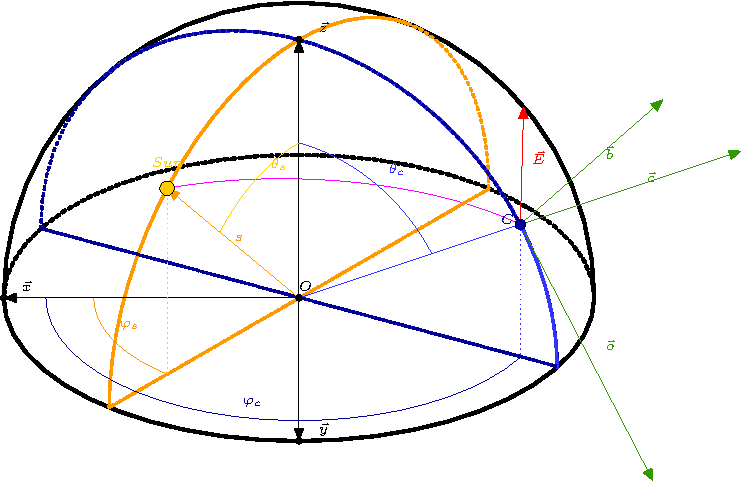
\includegraphics[width=0.4\textwidth]{./content/intro/figures/polasky4-crop.pdf}
  \label{fig:scattering}
  \caption{Skylight polarization by scattering\textcolor{red}{The figure needs
      to be re-designed according the text, and the yellow color is not readable}}
\end{figure}
Accordingly the normalized electric field vector $\vec{E}$ in the world frame
is presented as the normalized cross product of $\vec{s}$ and
$\vec{c}$ (see Eq.~\ref{Eq:E}).

\begin{equation}
\vec{E}=\frac{\vec{s}\wedge \vec{c}}{\left\Vert \vec{s}\wedge
    \vec{c}\right\Vert }
\label{Eq:E}
\end{equation}
The same measure in the pixel frame $\mathcal{P}$ ($\widehat{obc}$) is represented as:
% However measuring the skylight polarization pattern and \gls{aop}, the electric
% field in the pixel frame $\mathcal{P}$ ($\widehat{obc}$) is represented as:

\begin{equation}
E_{obc}=\left[\begin{array}{l}
E_{o}\\
E_{b}\\
0
\end{array}\right]=\left[\begin{array}{l}
\cos\alpha\\
\sin\alpha\\
0
\end{array}\right]
\label{Eq:Eproj}
\end{equation}
\noindent where $\alpha$ is the measured \gls{aop}.
Combination of Eq.~\ref{Eq:E}~\&~\ref{Eq:Eproj} and using the
scattering angle $\gamma$, between $\vec{s}$ and $\vec{c}$ leads to:
\begin{equation}
  \begin{cases}
(s\wedge c)\cdot o & =\sin\gamma\cos\alpha\\
(s\wedge c)\cdot b & =\sin\gamma\sin\alpha
\end{cases}
\label{eq:E0EB vect-1-1}
\end{equation}

\noindent applying vector triplet cross product rule on Eq.~\ref{eq:E0EB
  vect-1-1} results.
\begin{equation}
\begin{cases}
s\cdot b & =\sin\gamma\cos\alpha\\
s\cdot o & =-\sin\gamma\sin\alpha
\end{cases}
\label{eq:scal-b-o}
\end{equation}

Using Eq.~\ref{eq:3}, the scattering angle $\gamma$, therefore can be
represented as:
\begin{equation}
\cos\gamma=s\cdot c=\pm\sqrt{\frac{1-\rho_{l}'}{1+\rho_{l}'}}
\label{Eq:cosg}
\end{equation}
\noindent with $\rho_{l}'=\frac{\rho_{l}}{\rho_{l_{max}}}.$ \\
\vspace{0.4mm}
%\vskip{0.1mm}

Equations~\ref{eq:scal-b-o}~\&~\ref{Eq:cosg} finally leads to the sun vector
in pixel frame $\mathcal{P}$ which express a direct relation between the
measured polarization parameters (\gls{aop} and \gls{dopl}),
scattering angle, the sun position,  and the celestial point:
\begin{equation}
  \label{eq:sunp}
  \vec{s}_{p} =
    \begin{bmatrix}
    -\sin\gamma \sin\alpha\\
    \sin\gamma \cos\alpha\\
    \cos\gamma
  \end{bmatrix}
\end{equation}

\subsection{UAV attitude and polarized sky pattern}
\label{subsec:ps-attitude}
This section presents how the information presented so far can be used for
attitude estimation of a \gls{uav}.
The overview of the considered scenario, the frame conventions and rotations
for an \gls{uav} is shown in Fig.~\ref{fig:rotation}.

\begin{figure}[h]
  \centering
  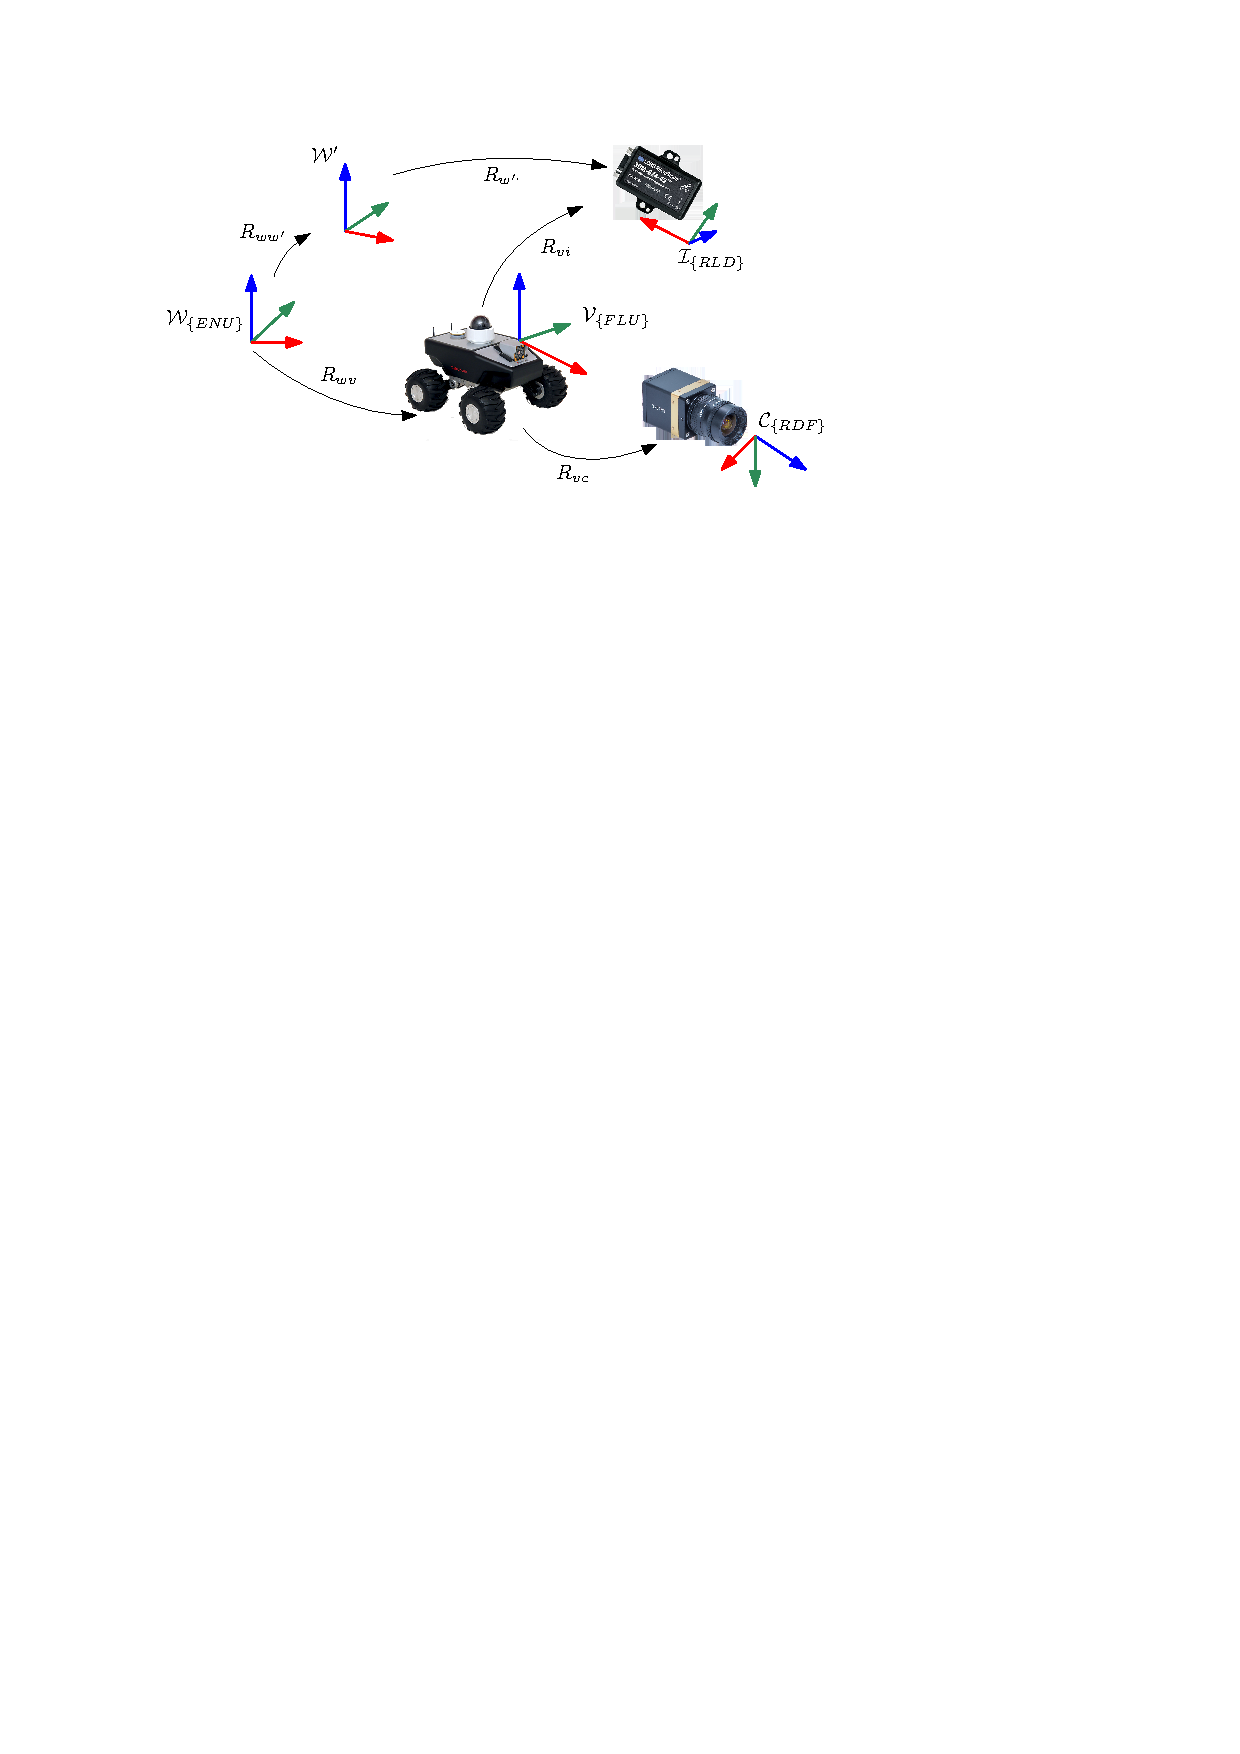
\includegraphics[width=0.5\textwidth]{./content/intro/figures/conventions.pdf}
  \label{fig:rotation}
  \caption{Frame conventions and rotations for attitude estimation of an
    \gls{uav}- \textcolor{red}{-the figure needs to be changed pixel frame
    should be added, some parts can be removed.}}
\end{figure}
In Fig.~\ref{fig:rotation} the $\mathcal{W}, \mathcal{W'}, \mathcal{I},
\mathcal{V}, \mathcal{C},$ and $\mathcal{P}$, present the world frame, global
frame of \gls{imu}, \gls{imu} frame, vehicle frame, camera frame, and pixel
frame respectively. Where the rotation from each frame to another is presented
with lowercase alphabet.
In the shown scenario, a vector $v_{p}$ in pixel frame is
expressed in the world frame, $v_{w}$:
\begin{equation}
  \label{eq:vinW}
  v_{w} = R_{wv} \cdot R_{vc} \cdot R_{cp} \cdot v_{p}
\end{equation}
\noindent where the rotation from the camera to the pixel frame $R_{cp}$ is
defined as the yaw and pitch rotation by the zenith and azimuth angle of the
celestial point ($\theta_c, \phi_c$) as shown in Eq.~\ref{eq:Rcp}.
\begin{equation}
  \label{eq:Rcp}
  \begin{split}
  R_{cp}  & =
  \begin{bmatrix}
    \cos\theta_{c}\cos\phi_{c} & -\sin\phi_{c} & \sin\theta_{c}\cos\phi_{c}\\
    \cos\theta_{c}\sin\phi_{c} & \cos\phi_{c} & \sin\theta_{c}\sin\phi_{c}\\
    -\sin\theta_{c} & 0 & \cos\theta_{c}
  \end{bmatrix}
  \\
  & = R_{z_{c}}(\phi_{c})\cdot R_{y_{c}}(\theta_{c})
  \end{split}
\end{equation}

Previously we presented how to express sun position in pixel frame (see
Eq.~\ref{eq:sunp}). Indeed this representation is applied to any point from
world frame, ergo:
\begin{equation}
  \label{eq:Rwv}
  \begin{split}
    s_{w} & = R_{wv} \cdot R_{vc} \cdot R_{cp} \cdot
    \begin{bmatrix}
    -\sin\gamma \sin\alpha\\
    \sin\gamma \cos\alpha\\
    \cos\gamma
  \end{bmatrix} = R_{wv} \cdot R_{vc} \cdot v\\
    & R^{T} \cdot s_{w}  = v
  \end{split}
\end{equation}

In the above equation, $\alpha$, $R_{cp}$, and $R_{vc}$ are known, however to
find the $R_{wv}$, $\gamma$ should be estimated. How to estimate this parameter
and definition of absolute and relative attitude estimation is explained in
next Sect.~\ref{sec:g-abs-rel}.





% Some stuff that emac's colegues use
%%% Local Variables:
%%% mode: late
%%% TeX-master: "../../main.tex"
%%% End: \section{Polarized cues used for attitude estimation}
